%%===========================================================%%
%%                                                           %%
%%                  ENERGY LOSS  CORRECTION                   %%
%%                                                           %%
%%===========================================================%%


\chapter{Energy Loss Correction}\label{chap:energyLossCorrection}
Particles passing through the detector material loose energy as they travel. The track momentum $p_T^{true}$ is reconstructed by fitting a helical path to the track points left in the detector. For this procedure all particles are assumed to be pions and the reconstructed momentum $p_T^{meas}$ is corrected by the amount of energy loss for a pion. Fitting the track points to an ideal
helical track tends to underestimate the momentum due to these energy loss efects. For kaons and protons ( or anything that is not a pion ) the amount of energy loss can be determined from simulated tracks run through GEANT.
The correction $p_T^{meas}-p_T^{true}$ was calculated for each particle species as a function of $p_T^{meas}$, $\eta$ and $z$-vertex. The energy loss correction averaged over $|\eta|<0.7$ for $K^-$ is shown in Fig. \ref{fig:energyLossPrimaryK_minus}. One can notice an offset of about $3-4$~MeV for negative $z$-vertex. It is a known issue with STAR simulation where HFT support material is badly described for negative $z<-30$~cm.
\noindent The energy loss corrections for other particle species are shown in \Cref{fig:energyLossPrimaryPi_minus,fig:energyLossPrimaryPi_plus,fig:energyLossPrimaryK_plus,fig:energyLossPrimaryP_bar,fig:energyLossPrimaryP,fig:energyLossPrimaryNegative,fig:energyLossPrimaryPositive} in Appendix \ref{appendix:energyLoss}.\newline
\noindent One may need the energy loss correction for reconstructed global proton and antiproton tracks to estimate the~knock-out proton background. During the reconstruction, global tracks are corrected only for energy losses in TPC, whereas primary tracks have the information of dead material inside and in front of TPC. Since that, there is an offset of about $4$~MeV for global tracks, what is shown in \Cref{fig:energyLossPrimaryP_barGlobal,fig:energyLossPrimaryPGlobal} in Appendix \ref{appendix:energyLoss}.


\begin{figure}[hb]
\caption[Energy loss correction for $K^-$ as a function of reconstructed transverse momentum $p_T^{meas}$.]{Energy loss correction $p_T^{meas}-p_T^{true}$ for $K^-$ as a function of reconstructed transverse momentum $p_T^{meas}$ $\left(|\eta|<0.7\right)$ in single $z$-vertex bin whose range is given on each plot.}\label{fig:energyLossPrimaryK_minus}
\centering
\parbox{0.329\textwidth}{
  \centering
  \includegraphics[width=\linewidth,page=23]{graphics/energyLoss/energyLoss3D_OnePrtAlso.pdf}\\
  \includegraphics[width=\linewidth,page=26]{graphics/energyLoss/energyLoss3D_OnePrtAlso.pdf}\\
  \includegraphics[width=\linewidth,page=29]{graphics/energyLoss/energyLoss3D_OnePrtAlso.pdf}\\
  \includegraphics[width=\linewidth,page=32]{graphics/energyLoss/energyLoss3D_OnePrtAlso.pdf}\\
}~
\parbox{0.329\textwidth}{
  \centering
  \includegraphics[width=\linewidth,page=24]{graphics/energyLoss/energyLoss3D_OnePrtAlso.pdf}\\
  \includegraphics[width=\linewidth,page=27]{graphics/energyLoss/energyLoss3D_OnePrtAlso.pdf}\\
  \includegraphics[width=\linewidth,page=30]{graphics/energyLoss/energyLoss3D_OnePrtAlso.pdf}\\
  \includegraphics[width=\linewidth,page=33]{graphics/energyLoss/energyLoss3D_OnePrtAlso.pdf}\\
}%
\parbox{0.329\textwidth}{
  \centering
  \includegraphics[width=\linewidth,page=25]{graphics/energyLoss/energyLoss3D_OnePrtAlso.pdf}\\
  \includegraphics[width=\linewidth,page=28]{graphics/energyLoss/energyLoss3D_OnePrtAlso.pdf}\\
  \includegraphics[width=\linewidth,page=31]{graphics/energyLoss/energyLoss3D_OnePrtAlso.pdf}\\
  \includegraphics[width=\linewidth,page=34]{graphics/energyLoss/energyLoss3D_OnePrtAlso.pdf}\\
}%
\end{figure}
\begin{figure}[H]\ContinuedFloat
% ~\\[32pt]
\parbox{0.329\textwidth}{
  \includegraphics[width=\linewidth,page=35]{graphics/energyLoss/energyLoss3D_OnePrtAlso.pdf}\\
}~
\parbox{0.329\textwidth}{
  \includegraphics[width=\linewidth,page=36]{graphics/energyLoss/energyLoss3D_OnePrtAlso.pdf}\\
}%
\parbox{0.329\textwidth}{
  \includegraphics[width=\linewidth,page=37]{graphics/energyLoss/energyLoss3D_OnePrtAlso.pdf}\\
}%
\end{figure}
\vspace{-3.5em}
\begin{figure}[H]\ContinuedFloat
% ~\\[32pt]
\parbox{0.329\textwidth}{
  \includegraphics[width=\linewidth,page=38]{graphics/energyLoss/energyLoss3D_OnePrtAlso.pdf}\\
}~
\end{figure}